%% The following is a directive for TeXShop to indicate the main file
%%!TEX root = diss.tex

\chapter{Methods}
\label{ch:Methods}

The simulation of the ARICH detector was created using \textsc{ROOT}: an object-oriented scientific computing framework based off C++ and developed at CERN \cite{root}.
\textsc{ROOT} is used for its ease of use, the high degree of organization and extensibility that comes from its object-oriented nature, and its high efficiency when compiled.
\textsc{PROOF} is an extension to \textsc{ROOT} that allows for parallelization of the code. The simulation was created in steps of increasing added complexity, which are outlined in this chapter.


\section{Initial Simulation}
\label{sec:experiment}
The first step in building the simulation was to generate particles, and have each of them generate photons at the appropriate angle as they travel through a single layer of aerogel. If we define the $z$ axis to be the downstream direction, then the inputs to the simulation are:
\begin{itemize}
\item The $x$ and $y$ position of a particle as it enters the aerogel.
\item The error on the $x$ and $y$ position of the particle, corresponding to the position resolution of the upstream particle tracker.
\item The $x$ and $y$ components of the unit vector representing the direction of the particle.
\item The error on the $x$ and $y$ direction of the particle, corresponding to the direction resolution of the upstream particle tracker.
\item The velocity $\beta$ of the particle.
\end{itemize} 
We generate 10,000 such particles whose positions and directions are randomly drawn from a Gaussian distribution with the specified mean values and errors. 
Each of these particles generates a number of photons equal to the result of equation \ref{eq:photonNumber} multiplied by the distance the particle has to travel through the aerogel.
These photons are randomly distributed along the path travelled by the particle. Their polar angle $\theta$ with respect to the direction of travel of the particle is given by equation \ref{eq:cherenkovAngle}, and their azimuthal angle is randomly drawn from between 0 and $2\pi$. 
If we are given the direction vector of the particle, we can use a rotation matrix to get the resulting direction vectors for each of the photons it generates.
This is given by \TODO{RODRIGUES' ROTATION FORMULA}

Each photon is generated with a corresponding wavelength, drawn randomly from \TODO{INTEGRATE FRANK TAMM}. 
Given the point of generation and the direction vector of each photon, we can then determine where on the aerogel the photon will hit.
We then apply efficiency corrections to see whether the photon would be registered as a hit: \TODO{EXPLAIN DETECTOR FILL EFFICIENCY}.
We also know the quantum efficiency of the PMTs across different photon wavelengths, so we can throw out photons randomly by their wavelength.

\section{Optical Effects}

Once this simple simulation has been verified, the effects of photon scattering in the aerogel will be incorporated into the simulation.
The transmittance of these photons through the aerogel has contributions from scattering and absorption effects, but the dominant contribution is from Rayleigh scattering \cite{aerogelRefraction}.
The probability that a photon  undergoes Rayleigh scattering is proportional to $\lambda^{-4}$, where $\lambda$ is the wavelength of the light, and the angular distribution of scattered photons is proportional to $1 + \cos^2(\theta)$ \cite{rayleigh}.
The known optical transmittance of the aerogel \cite{aerogelRefraction} may be fit to obtain the probability that a photon will undergo Rayleigh scattering after travelling some distance.
We enhance our simulation by adding this random scattering effect to each photon: we randomly select whether the photon will have scattered at each point in its trajectory based off this probability, and generate a new $\theta$ and $\phi$ for the photon. 

After simulating thousand of particles entering the \ac{ARICH} with a given velocity and trajectory, we can average over all the photons hitting the detector to get a probability distribution.
An example of a probability distribution is shown in Figure \ref{fig:particleRings}.
This probability distribution can then be used for particle identification.

\begin{figure}[h!]
\centering
\resizebox{0.8\textwidth}{!}{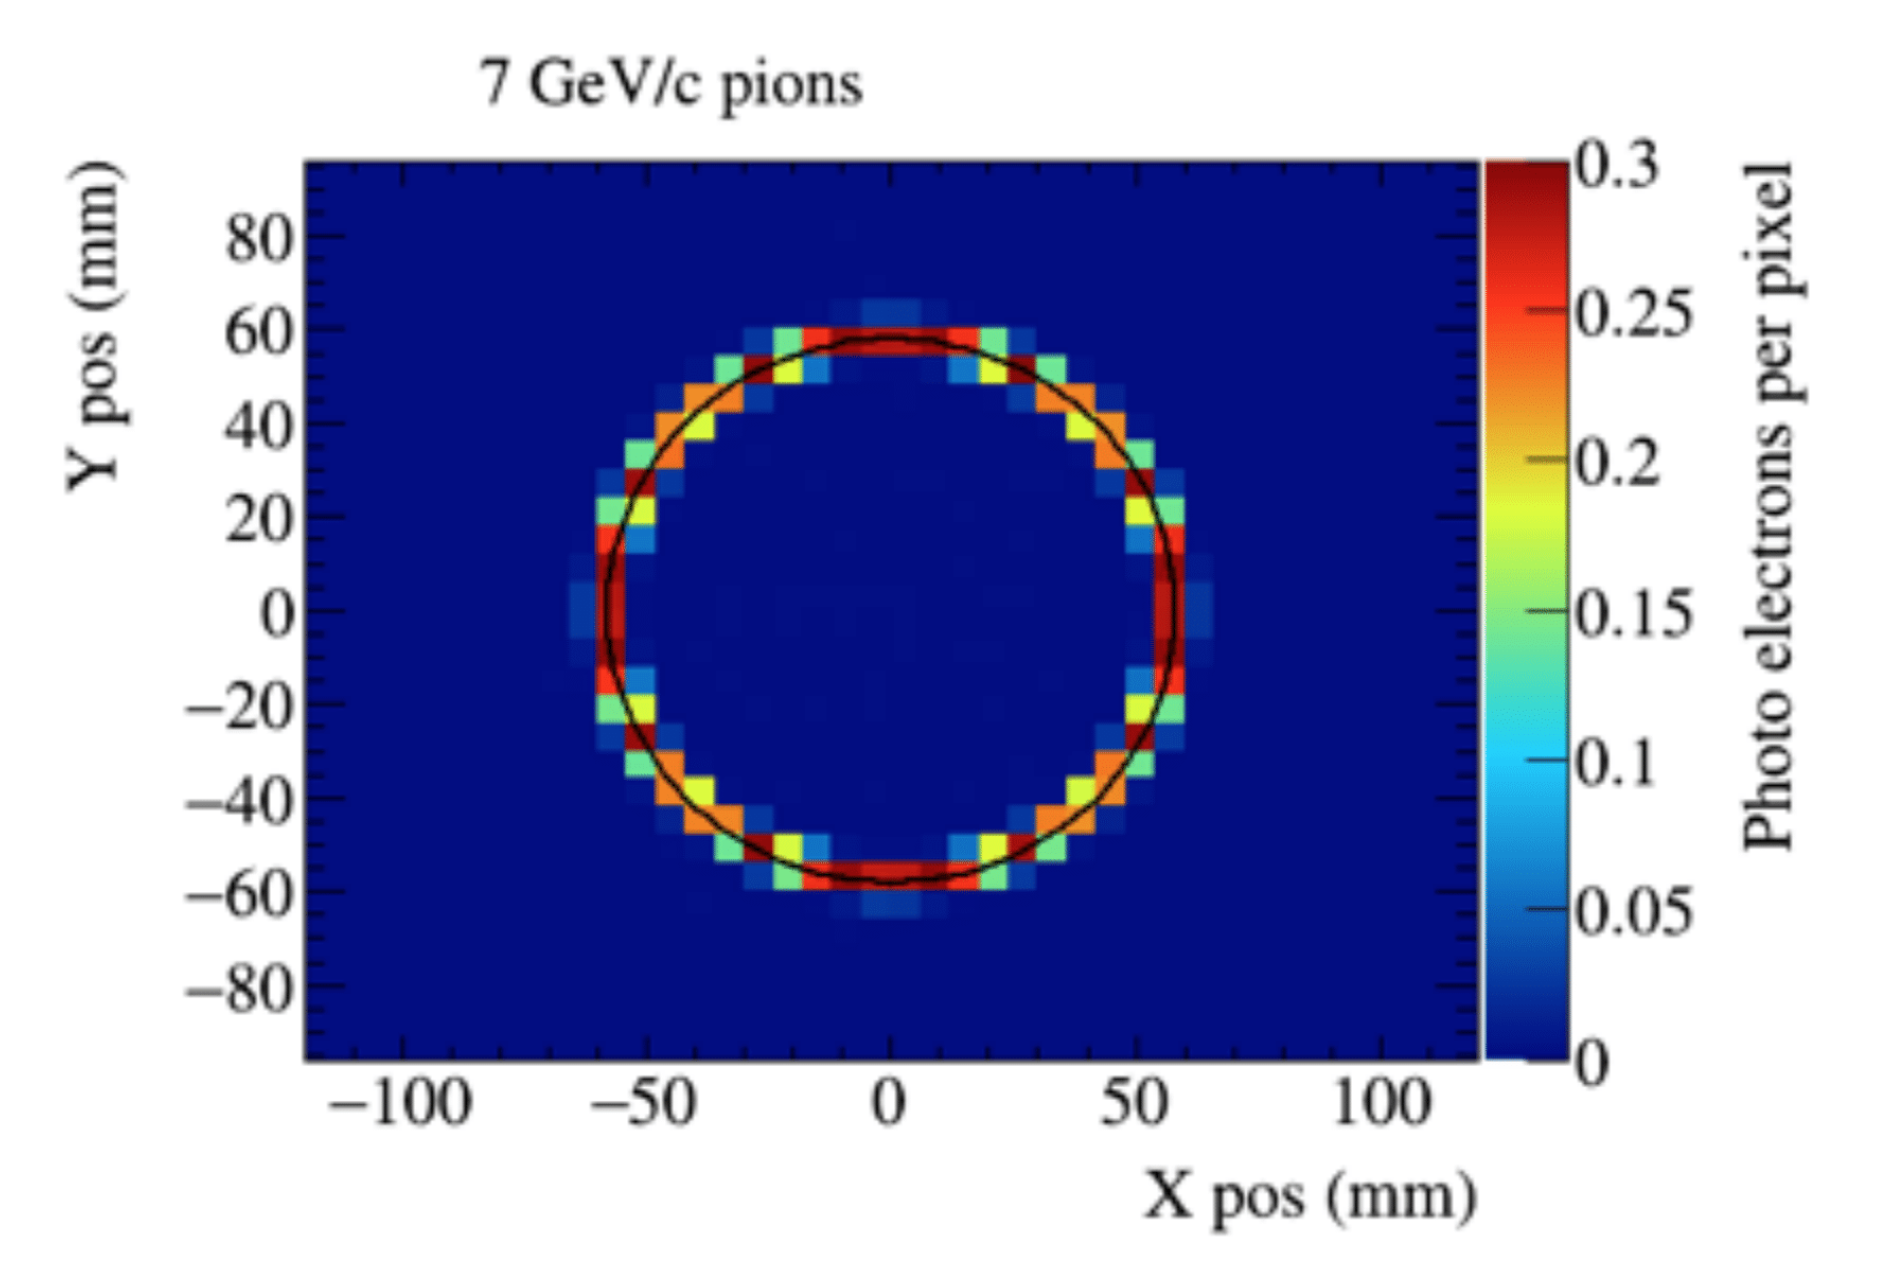
\includegraphics{./figs/particleRing.png}}
\caption[Example of a simulated photon probability distribution]{Example of the photon probability distribution on a detector plane resulting from a simulation of the photons emitted by 10,000 pions with a momentum of 7 GeV/c emitting Cherenkov radiation. The photons were simulated using \textsc{Geant4}. The figure was obtained with permission from the \textsc{EMPHATIC} group.}

\label{fig:particleRings}       % Give a unique label to the figure. 
\end{figure}

Once a simulation has been created to handle this procedure, it will be verified against an already-existing simulation of the full detector configuration.
The full simulation is handled with \textsc{Geant4}, a C++ based software toolkit designed for Monte Carlo simulations of particles travelling through complex detector geometry  \cite{geant4}.

\section{Particle Identification}
\label{sec:particleIdentification}
In order to identify particles using the \ac{ARICH} detector, a particle likelihood method is used \cite{richImpact, belleArich}.
For this method, we take the known momentum of the particle, and use Equation \ref{eq:relMass} to determine the expected velocity for different candidate particles masses.
The candidate particles of interest to the experiment are protons, electrons, pions, and kaons.
For each velocity hypothesis, we run 10,000 simulations of particles moving at that velocity, with the same measured initial trajectory as input.
For each pixel of the detector, this procedure will give a value $\lambda_i(\beta)$, equal to the expected number of photons striking pixel $i$ in the detector due to a particle of velocity $\beta$. 

For a given particle event, we will detect $N_i$ photons in each pixel $i$.
In reality, the PMTs are only capable of registering whether or not a photon has been detected - if multiple photons strike a single pixel in a very short amount of time, it will not be able to distinguish the number detected, so we just know if $N_i = 0$ or $N_i > 0$.

The probability that zero photons strike pixel $i$ is given by the Poisson distribution for zero events:
$$ P_i(N_i=0; \beta) = e^{-\lambda_i(\beta)} $$
 The probability that one or more photons strike pixel $i$ must then be:
$$ P_i(N_i>1; \beta) = 1 - e^{-\lambda_i(\beta)} $$

By multiplying the probabilities of getting the observed result in each pixel $i$ of the detector, we calculate the likelihood for that value of $\beta$:

$$L_\beta = \prod_{i}P_i(N_i; \beta)$$

For convenience, we actually compute:
\begin{equation}
    \label{eq:loglikelihood}
    -2\ln(L_\beta) = \sum_i \ln(P_i(N_i; \beta))
\end{equation}


We compute the log-likelihood of our data matching each of particle hypothesis, and choose that which minimizes the value.

\section{Multiparticle events};




\endinput

Any text after an \endinput is ignored.
You could put scraps here or things in progress.
